\documentclass{report}

\input{preamble}
\input{macros}
\input{letterfonts}

\title{\Huge{Math 120}}
\author{\huge{PSet 7}}
\date{Oct 24 2024}

\begin{document}

\maketitle
\newpage% or \cleardoublepage
% \pdfbookmark[<level>]{<title>}{<dest>}
\pdfbookmark[section]{\contentsname}{toc}
\tableofcontents
\pagebreak

\chapter{}
\section{PSet 7}

\qs{}{
    Calculate the given iterated integrals.
    \begin{enumerate}
        \item \( \int_0^1 \int_0^1 x \sqrt{1 + 4y} \, dy \, dx \)
        \item \( \int_0^1 \int_1^2 \frac{xe^x}{y} \, dy \, dx \)
    \end{enumerate}
}

\sol{
    \\
    1) 
    \[ \int_{0}^{1} \int_{0}^{1} x \sqrt{1 + 4y} \, dy \, dx \] 
    \[ \int_{0}^{1} x \sqrt{1 + 4y} \, dy \]
    \[ 1 + 4y = t \quad r = dt \]
    \[ x \int_{0}^{1} \frac{1}{4} \sqrt{t} dt \] 
    \[ \frac{1}{4}x \int_{0}^{1} \sqrt{t} dt \]  
    \[ \left. \frac{1}{4}x \cdot \frac{2t\sqrt{t}}{3} \right|_{0}^{1} \]
    \[ \left. \frac{1}{4}x \cdot \frac{2(1 + 4y)\sqrt{1+4y}}{3} \right|_{0}^{1} \]
    \[ \left. \frac{x\sqrt{1+4y}(1+4y)}{6} \right|_{0}^{1} \] 
    \[ \frac{x \sqrt{1+4}(1+4)}{6} - \frac{x\sqrt{1}{1}}{6} \] 
    \[ \frac{5x\sqrt{5}}{6} - \frac{x}{6} \] 
    \[ \int_{0}^{1} \frac{5x\sqrt{5}}{6} - \frac{x}{6} dx \] 
    \[ \frac{1}{6} \int_{0}^{1} 5\sqrt{5}x - x \, dx \] 
    \[ \frac{1}{6}\left(\int_{0}^{1} 5\sqrt{5} x dx - \int_{o}^{1} x \, dx \right)\]
    \[ \int_{0}^{1} 5 \sqrt{5}x \, dx \Rightarrow \left. \frac{5 \sqrt{5}x^{2}}{2} \right|_{0}^{1} \] 
    \[ \frac{5 \sqrt{5} (1)^{2}}{2} - 0  = \frac{5\sqrt{5}}{2} \] 
    \[ \int_{0}^{1} x \, dx \Rightarrow \left. \frac{x^{2}}{2} \right|_{0}^{1}\]  
    \[ \frac{1}{2} - 0 = \frac{1}{2}\] 
    \[ \frac{1}{6}\left( \frac{5\sqrt{5}}{2} - \frac{1}{2} \right) = \frac{5\sqrt{5} - 1}{12} \] 
    2) 
    \[ \int_{0}^{1} \int_{1}^{2}  \frac{xe^{x}}{y} \, dy \, dx \]
    \[ xe^{x} \int_{1}^{2} \frac{1}{y} \, dy \]
    \[ xe^{x} \left. \ln(y) \right|_{1}^{2} \Rightarrow xe^{x} \ln(2) - xe^{x}\ln(1) = xe^{x} \ln(2)\] 
    \[ \ln(2) \int_{0}^{1} xe^{x} \, dx  \]
    \[ \ln(2) \left. \left(xe^{x} -e^{x} \right) \right|_{0}^{1} \] 
    \[ \left(\ln(2)e - \ln(2)e \right) - \left(\ln(2)(0) - \ln(2)e^{0} \right) = 0 - (-\ln(2)(1)) = \ln(2) \]    
}

\qs{}{
    \begin{enumerate}
        \item[(a)] Sketch the solid whose volume is given by the iterated integral 
        \[ \int_0^1 \int_0^2 e^{-x^2 - y^2} \, dy \, dx. \]

        \item[(b)] Explain why 
        \[ \int_0^1 \int_0^2 e^{-x^2 - y^2} \, dy \, dx = \int_0^1 e^{-x^2} \, dx \cdot \int_0^2 e^{-y^2} \, dy. \]

        \item[(c)] Use Desmos to compute 
        \[ \int_0^1 \int_0^2 e^{-x^2 - y^2} \, dy \, dx. \]
        (Desmos will give a numerical approximation, but this is fine. In fact, there is no way to compute the antiderivatives necessary to get an exact answer.)
    \end{enumerate}
}

\sol{
    \begin{center}
        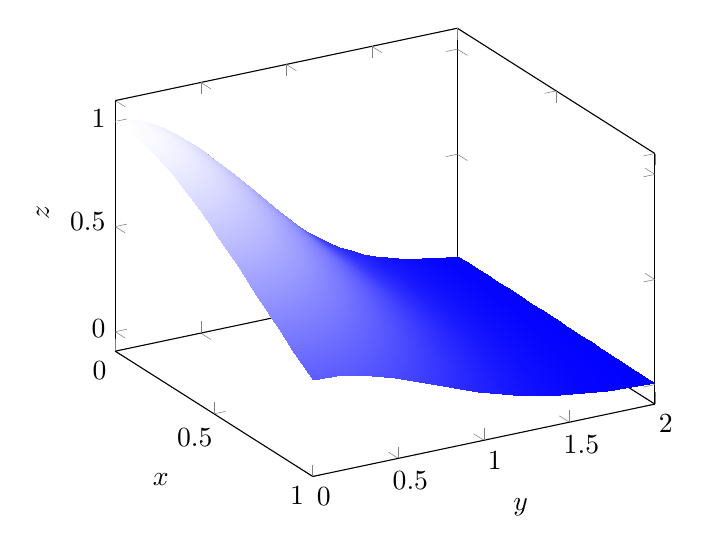
\begin{tikzpicture}
            \begin{axis}[
              view={60}{30}, 
              xlabel={$x$}, ylabel={$y$}, zlabel={$z$},
              domain=0:1, y domain=0:2,
              samples=30,
              colormap/viridis,
              mesh/interior colormap={bluewhite}{color=(blue) color=(white)},
              ]
              \addplot3[surf, shader=interp] 
              {exp(-x^2 - y^2)};
            \end{axis}
          \end{tikzpicture}       
    \end{center}
}

\qs{}{
    \begin{enumerate}
        \item[(a)] Find the average value of the function \( f(x, y) = \sin x \cos y \) on the rectangle \( R = [0, \pi] \times [-\pi/2, \pi/2]. \)
        
        \item[(b)] Use symmetry to find the average value of \( f(x, y) = \frac{4 \sin y}{e^{x^2}} - \frac{\cos x}{\ln y} + 3 \) on the region \( R = [2\pi, 4\pi] \times [2\pi, 6\pi]. \) Please explain your answer carefully.
    \end{enumerate}
}

\sol{
    a) 
    \[ f(x,y) = \sin x \cos y \]
    \[ R = [0, \pi ] \times [- \frac{\pi}{2}, \frac{\pi}{2}] \]
    \[ f_{avg} = \frac{1}{A(R)} \iint\limits_{R} f(x,y) dA \]
    \[ A(R) = (\pi - 0 ) \times (\frac{\pi}{2} - -\frac{\pi}{2}) = \pi^{2} \] 
    \[ \frac{1}{\pi^{2}} \int_{0}^{\pi} \int_{-\frac{\pi}{2}}^{\frac{\pi}{2}} \sin x \cos y  \, dy \, dx \] 
    \[ \sin x \int_{-\frac{\pi}{2}}^{\frac{\pi}{2}} \cos y \, dy \]
    \[ \left. (\sin x) \sin y \right|_{\frac{pi}{2}}^{\frac{\pi}{2}} \]  
    \[ (\sin x )\sin\left(\frac{\pi}{2}\right) - (\sin x )\sin\left(\frac{- \pi}{2}\right) = 2 \sin x \] 
    \[ \int_{0}^{\pi} 2 \sin x dx \]
    \[ \left. -2 \cos x \right|_{0}^{\pi} \]
    \[ -\cos \pi - (-2)\cos(0) = 4 \]
    \[ \frac{1}{\pi^{2}} \cdot 4 = \frac{4}{\pi^{2}} \]    
    b) 
    \[ f(x,y) = \frac{4 \sin y}{e^{x^{2}}} - \frac{\cos x}{\ln y} + 3 \]
    \[ R = [2 \pi, 4 \pi ] \times [2\pi, 6 \pi] \]
    \[ f_{avg} = \iint\limits_{R} f(x,y) dA \] 
    \[ A(R) = [4 \pi - 2 \pi ] \times [6\pi - 2 \pi] = 8 \pi^{2} \] 
    \[ \int_{2\pi}^{4 \pi} \int_{2 \pi}^{6 \pi} \frac{4 \sin y}{e^{x^{2}}} - \frac{\cos x}{\ln y }  + 3 \, dy \, dx \]
    \[ \iint\limits_{R} f(x,y) dA  - \iint\limits_{R} \frac{4 \sin y}{e^{x^{2}}} dA - \iint\limits_{R} \frac{\cos x}{\ln y } dA  + \iint\limits_{R} 3 dA\] 
    \[ \int_{2\pi}^{6 \pi} 4 \sin y \, dy = -4\left[ \cos y\right]_{2 \pi}^{6 \pi} = -4(6 \cos \pi - \cos 2 \pi) = -4(1 - 1) = 0 \]
    \[ \iint\limits_{R} f(x,y) \frac{4 \sin y}{e^{x^{2}}} dA = \int_{2 \pi}^{4 \pi} \frac{1}{e^{x^{2}}}dx \times 0 = 0 \]
    \[ \int_{2 \pi}^{4 \pi} {\cos x} dx = \left. \sin x \right|_{2 \pi}^{4 \pi} = sin 4 \pi - \sin 2 \pi = 0 - 0 = 0\] 
    \[ \iint\limits_{R} \frac{\cos x}{\ln y } dA = \int_{2 \pi}^{6 \pi} \frac{1}{\ln y} \times 0 = 0 \] 
    \[ \iint\limits_{R} 3 dA = 3 \times A(R) = 3 \times 8 \pi^{2} = 24 \pi^{2} \]
    \[ \frac{24 \pi^{2}}{8 \pi^{2}} = 3 \]  
}

\qs{}{
    In each part, draw the region \( D \), and evaluate the integral.
    \begin{enumerate}
        \item \( \iint_D \frac{y}{x^5 + 1} \, dA \), where \( D \) is the region \( D = \{(x, y) \mid 0 \leq x \leq 1, \, 0 \leq y \leq x^2 \}. \)
        \item \( \iint_D x^3 \, dA \), where \( D = \{(x, y) \mid 1 \leq x \leq e, \, 0 \leq y \leq \ln x \}. \)
    \end{enumerate}
}

\sol{
    1. 
    \[ \iint_D \frac{y}{x^5 + 1} \, dA  \quad D = \{(x, y) \mid 0 \leq x \leq 1, \, 0 \leq y \leq x^2 \} \]
    \[ \int_{0}^{1} \int_{0}^{x^{2}} \frac{y}{x^{5} + 1} \, dy \, dx \] 
    \[ \frac{1}{x^{5} + 1} \int_{0}^{x^{2}} y dy \]
    \[ \left. \frac{y^{2}}{2}\right|_{0}^{x^{2}} \Rightarrow \frac{\left(x^{2}\right)^{2}}{2} - \frac{0}{2} = \frac{x^{4}}{2} \]  
    \[ \int_{0}^{1} \frac{1}{x^{5} + 1} \times \frac{x^{4}}{2} dx \] 
    \[ x^{5} + 1 = t \quad dt = 5x^{4} dx \] 
    \[ \frac{1}{10} \int_{0}^{1} \frac{1}{t} dt \]
    \[ \left. \frac{1}{10} \ln|t| \right|_{0}^{1} \]
    \[ \left. \frac{1}{10} | x^{5} + 1 | \right|_{0}^{1} \]
    \[ \frac{1}{10} \ln(1^{5} + 1)   - \frac{1}{10}\ln(1) \]
    \[ \frac{1}{10} \ln(2) - \frac{1}{10} \ln(1) = \frac{1}{10} \ln(2) \]  
    2.    
}

\qs{}{
    Draw the region \( D \). Set up the iterated integrals for both orders of integration. 
    Then evaluate the double integral using the easier order and explain why it's easier.
    \[ \iint_D x^2 e^{-xy} \, dA \quad \text{where } D \text{ is bounded by } y = x, \, x = 4, \, \text{and } y = 0. \]
}

\qs{}{
    \begin{enumerate}
        \item[(a)] Find the volume of the solid in the first octant enclosed by the parabolic cylinder \( y = 1 - x^2 \) and the planes \( z = 2 - y \) and \( z = y \).
        
        \item[(b)] Sketch the solid whose volume is given by the iterated integral 
        \[ \int_0^1 \int_0^{1-x} (2 - y^2) \, dy \, dx. \]
    \end{enumerate}
}

\qs{}{
    Sketch the region of integration and change the order of integration.
    \begin{enumerate}
        \item \( \int_0^1 \int_{4x}^4 f(x, y) \, dy \, dx \)
        \item \( \int_0^3 \int_{\sqrt{9 - y}}^3 f(x, y) \, dx \, dy \)
        \item \( \int_0^4 \int_0^{\ln 2x} f(x, y) \, dy \, dx \)
    \end{enumerate}
}

\qs{}{
    Evaluate the integral 
    \[ \int_0^1 \int_x^1 \frac{e^x}{y} \, dy \, dx \]
    by reversing the order of integration.
}

\qs{}{
    Evaluate the given integral by converting to polar coordinates. Be sure to draw the region of integration in each part.
    \begin{enumerate}
        \item \( \iint_R (x + y) \, dA \), where \( R \) is the region that lies to the left of the \( y \)-axis between the circles \( x^2 + y^2 = 1 \) and \( x^2 + y^2 = 4 \).
        \item \( \iint_R y e^x \, dA \), where \( R \) is the region in the first quadrant enclosed by the circle \( x^2 + y^2 = 25 \).
    \end{enumerate}
}

\qs{}{
    Use polar coordinates to find the volume of the given solid.
    \begin{enumerate}
        \item[(a)] Inside the sphere \( x^2 + y^2 + z^2 = 4 \) and outside the cylinder \( x^2 + y^2 = 1 \).
        \item[(b)] Bounded by the paraboloids \( z = 3x^2 + 3y^2 \) and \( z = 4 - x^2 - y^2 \).
    \end{enumerate}
}

\qs{}{
    Evaluate the iterated integral 
    \[ \int_0^b \int_{-\sqrt{b^2 - y^2}}^0 x^2 y \, dx \, dy \]
    by converting to polar coordinates.
}

\qs{}{
    Let \( D \) be the disk with center at the origin and radius \( a \).
    \begin{enumerate}
        \item[(a)] Use your intuition: what do you expect is the average distance from points on the disk to the origin?
        \begin{itemize}
            \item less than \( a/2 \)
            \item \( a/2 \)
            \item between \( a/2 \) and \( a \)
            \item more than \( a \)
        \end{itemize}
        Give an intuitive explanation of your answer.

        \item[(b)] What is the average distance from points in the disk to the origin?
    \end{enumerate}
}

\end{document}
